\begin{frame}
\frametitle{Results}
\framesubtitle{GNTSAT (uniform crossover) vs WalkSAT}
\begin{tabular}{r | r r r | r r r}
	\hline
	      &      & GNTSAT                     &                     &      & WalkSAT                    &                     \\
	Suite & SR   & AFS \tiny{($\times 10^3$)} & AT \tiny{(seconds)} & SR   & AFS \tiny{($\times 10^3$)} & AT \tiny{(seconds)} \\
	\hline
	100   & 1.00 & 33.75                      & 0.18                & 1.00 & 28.89                      & 0.15                \\
	150   & 1.00 & 193.45                     & 1.48                & 1.00 & 123.73                     & 0.94                \\
	200   & 0.94 & 776.71                     & 7.81                & 0.90 & 1322.66                    & 13.27               \\
	250   & 0.92 & 2008.86                    & 25.07               & 0.40 & 5054.14                    & 63.38
\end{tabular}

\begin{alertblock}{Results}
	Significant difference in the benchmark suite with 250
	variables
	\begin{itemize}
		\item Much higher success rate (0.92 vs 0.40)
		\item Much less computation ($2.0 \times 10^6$ vs $5.1 \times 10^6$ flips)
	\end{itemize}
\end{alertblock}
\end{frame}

\begin{frame}
\frametitle{Results}
\framesubtitle{With different crossover operators}
\begin{figure}[htpb]
	\centering
	\includegraphics[scale=0.13]{AFS.png}
\end{figure}
\end{frame}

\begin{frame}
\frametitle{Results}
\framesubtitle{With different crossover operators}
\begin{figure}[htpb]
	\centering
	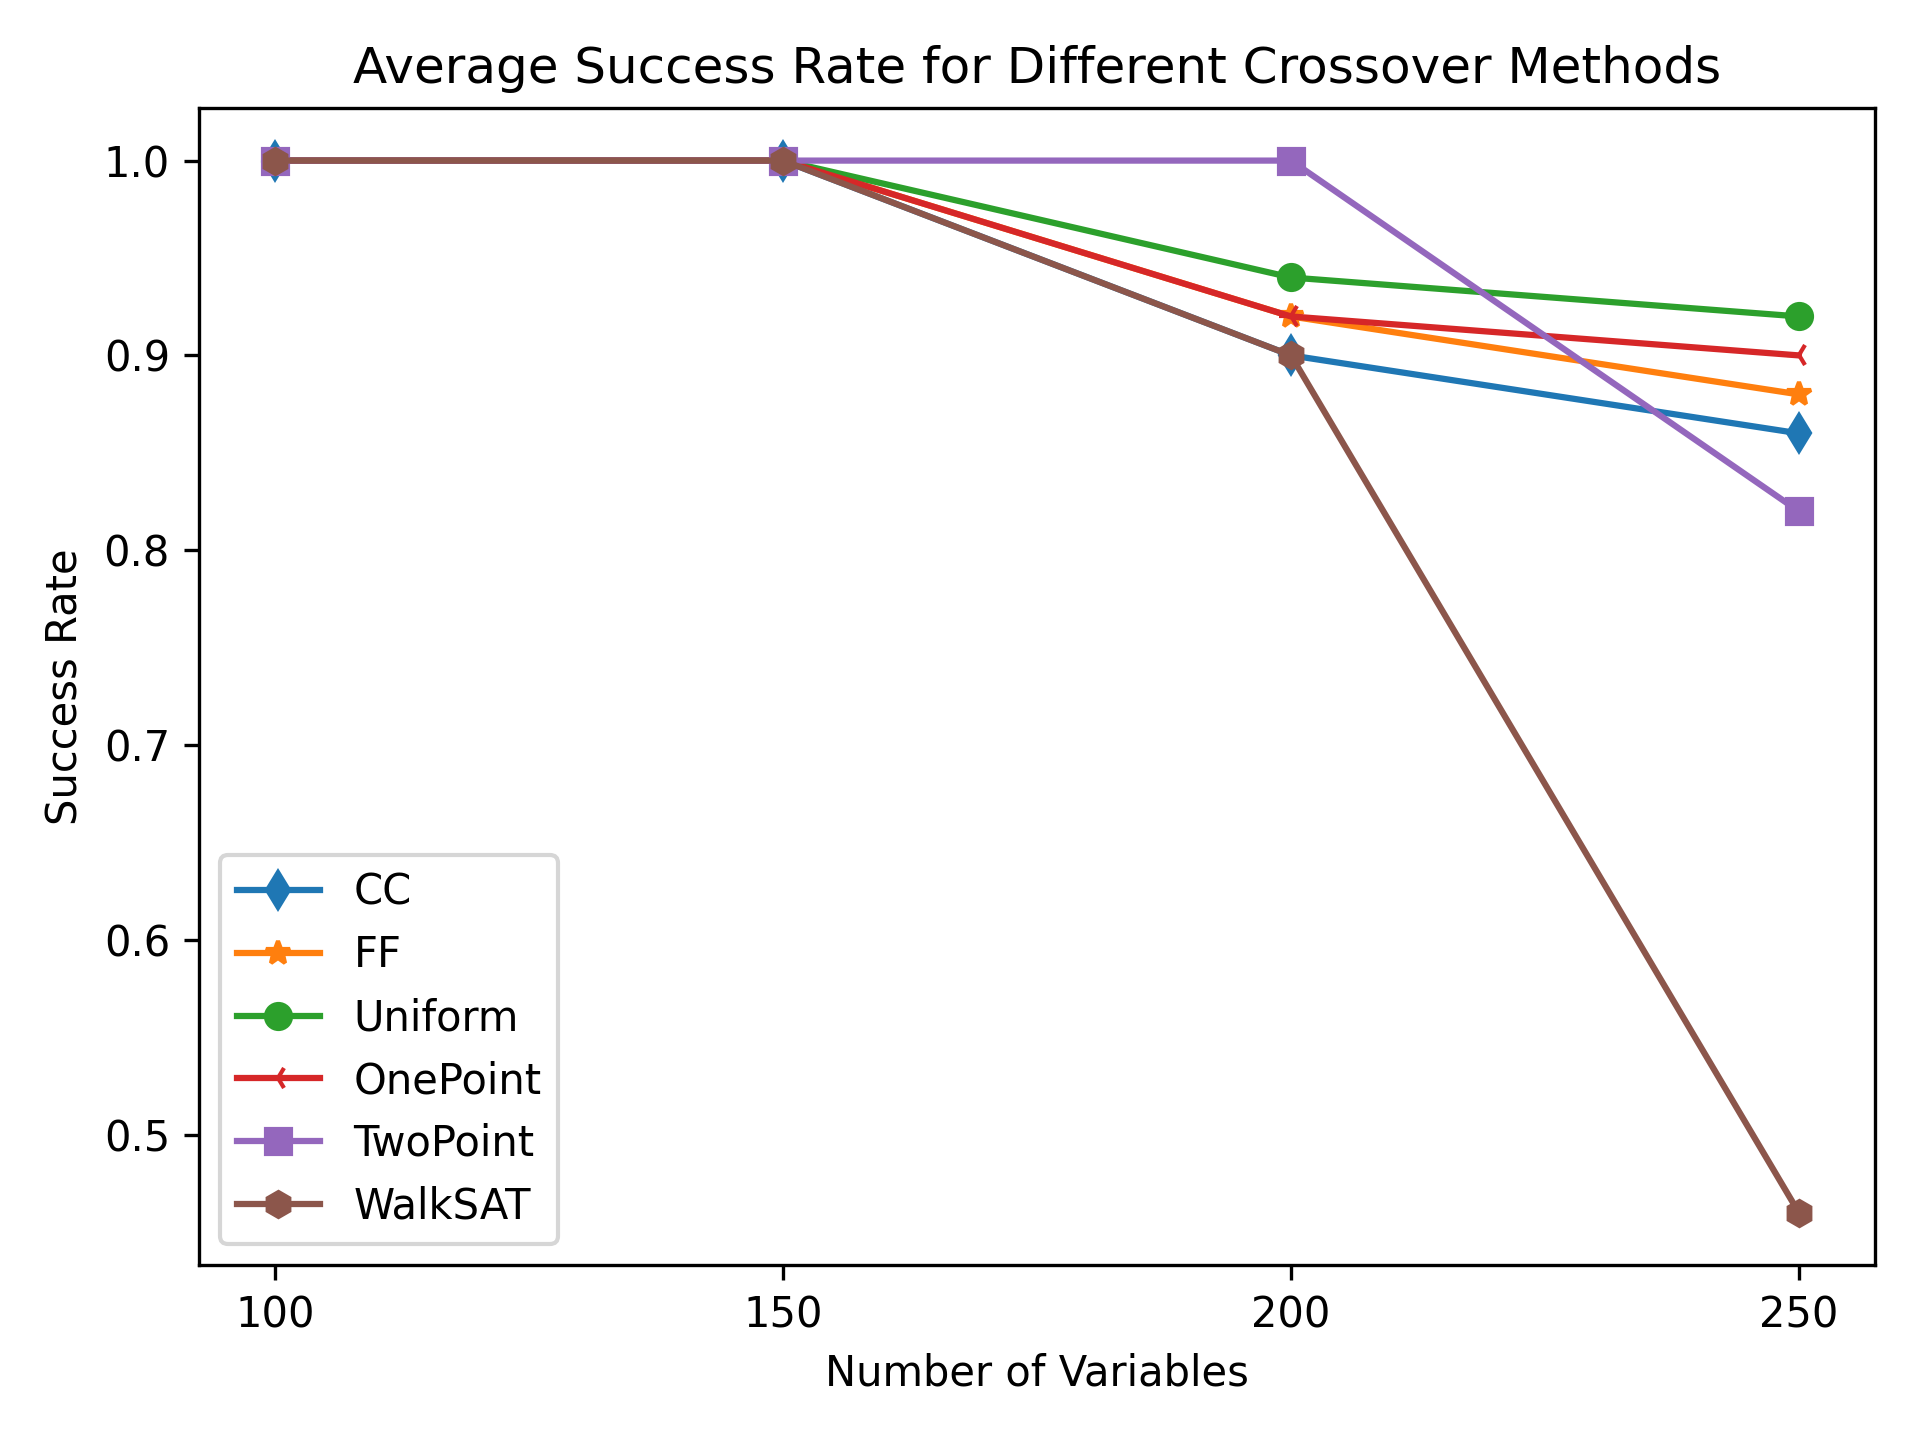
\includegraphics[scale=0.13]{AverageSR.png}
\end{figure}
\end{frame}

\begin{frame}
\frametitle{Results}
\framesubtitle{Summary}
\begin{alertblock}{GNTSAT vs WalkSAT}
	GNTSAT outperforms WalkSAT in terms of both success
	rate and computation on larger uniform random 3-SAT instances.
\end{alertblock}

\begin{alertblock}{Different crossover operators in GNTSAT}
	They perform similarly. Uniform crossover appears to
	be slightly more stable and faster on larger uniform random 3-SAT instances
	(needs to be confirmed by further studies).
\end{alertblock}

\end{frame}
